%\documentclass{sig-alternate-05-2015}
\documentclass{llncs}
\usepackage{makeidx}
\usepackage{tabularx,colortbl}
\usepackage[dvipsnames]{xcolor}
\usepackage{flushend}
\usepackage{cite}
\usepackage{amsmath}
%\usepackage{amsthm}
\usepackage{amssymb}
\usepackage{epsfig}
\usepackage{stmaryrd}
\usepackage{url}
\usepackage{multirow}
\usepackage{latexsym}
\usepackage{graphics}
\usepackage{graphicx}
\usepackage{enumitem}
\usepackage{comment}
\usepackage{longtable}
\usepackage{supertabular}
\usepackage{times}
\usepackage{listings}
\usepackage{subfigure}
\usepackage{color}
\usepackage{balance}
\usepackage{xspace}
\usepackage[ruled, vlined, linesnumbered]{algorithm2e}
\usepackage[autostyle]{csquotes}



%\theoremstyle{Definition}
%\newtheorem{definition}{Definition}
%%%
%\theoremstyle{Theorem}
%\newtheorem{theorem}{Theorem}


%\newcommand{\definition}{\noindent \textbf{Definition} \citation{}}
%\newcommand{\theorem}{\noindent \textbf{Theorem} \citation{}}
%\newcommand{\lemma}{\noindent \textbf{Lemma} \citation{}}

%\newdef{lemma}{Lemma}
%\newdef{definition}{Definition}
%\newdef{theorem}{Theorem}
%\newdef{corollary}{Corollary}
%\newdef{note}{Note}
%\newdef{axiom}{Axiom}
\newcommand{\mkeyword}[1]{\mbox{\texttt{#1}}}
\DeclareMathOperator{\kuop}{uop}
\DeclareMathOperator{\kbop}{bop}
\DeclareMathOperator{\kite}{ite}
\DeclareMathOperator{\kpre}{pre}
\DeclareMathOperator{\dom}{dom}
\DeclareMathOperator{\ktrue}{true}
\DeclareMathOperator{\kfalse}{false}
\DeclareMathOperator{\kselect}{select}
\DeclareMathOperator{\ran}{range}
\newcommand{\lbb}{[\![}
\newcommand{\rbb}{]\!]}
\newcommand{\expr}{\phi}
\newcommand{\exprS}{\Phi}
\newcommand{\mike}[1]{\textcolor{red}{#1}}
\newcommand{\mats}[1]{\textcolor{blue}{#1}}
\newcommand{\darren}[1]{\textcolor{green}{#1}}
\newcommand{\danielle}[1]{\textcolor{orange}{#1}}

\sloppypar



\begin{document}

\definecolor{gold}{rgb}{0.90,.66,0}
\definecolor{dgreen}{rgb}{0,0.6,0}
\newcommand{\stateequiv}{\equiv_{s}}
\newcommand{\traceequiv}{\equiv_{\sigma}}
\newcommand{\ta}{\text{TA}}
\newcommand{\cta}{\text{TA$_{C}$}}
\newcommand{\tta}{\text{TA$_{T}$}}
\newcommand{\ucalg}{\texttt{\small{IVC\_UC}}}
\newcommand{\ucbfalg}{\texttt{\small{IVC\_UCBF}}}


\title{Safety Annex for AADL}
%
\author{Danielle Stewart\inst{1}
\and Janet Liu\inst{2}
\and Michael W. Whalen\inst{1}
\and Darren Cofer\inst{2} }
\institute{University of Minnesota\\Department of Computer
Science and Engineering\\
200 Union Street\\
Minneapolis, MN, 55455, USA\\
\email{dkstewar, whalen@cs.umn.edu}
\and
Rockwell Collins\\
Advanced Technology Center\\400 Collins Rd. NE\\
Cedar Rapids, IA, 52498, USA\\ \email{ Jing.Liu, darren.cofer@rockwellcollins.com}
}
\maketitle

\begin{abstract}
This paper describes the Safety Annex for Architecture Analysis and Design Language (AADL). The safety annex provides model-based safety analysis features for systems which have been annotated with an Assume-Guarantee Reasoning Environment (AGREE). Using a quantitative reasoning approach, the safety annex provides a model-based safety analysis approach in which faults can be formalized and analyzed. The language for describing faults is extensible which allows safety engineers to weave various types of faults into the nominal system model. The safety annex supports the injection of faults into component level outputs and the behavior of the system can be analyzed using model checking support through AGREE. 


\end{abstract}

\keywords{Model-based systems engineering, fault analysis, safety engineering}

\section{Introduction}

System safety analysis techniques are well established and are a required activity in the development of commercial aircraft and safety-critical ground systems. However, these techniques are based on informal system descriptions that are separate from the actual system design artifacts, and are highly dependent on the skill and intuition of a safety analyst. The lack of precise models of the system architecture and its failure modes often forces safety analysts to devote significant effort to gathering architectural details about the system behavior from multiple sources and embedding this information in safety artifacts, such as fault trees.

While model-based development (MBD) methods are widely used in the aerospace industry, they are generally disconnected from the safety analysis process itself. Formal model-based systems engineering (MBSE) methods and tools~\cite{QFCS15:backes,hilt2013,NFM2012:CoGaMiWhLaLu,DBLP:journals/scp/CimattiT15,Pajic2012,DBLP:conf/adaEurope/SokolskyLC09} now permit system-level requirements to be specified and analyzed early in the development process. These tools can also be used to perform safety analysis based on the system architecture and initial functional decomposition. Design models from which aircraft systems are developed can be integrated into the safety analysis process to help guarantee accurate and consistent results. This integration is especially important as the amount of safety-critical hardware and software in domains such as aerospace, automotive, and medical devices has dramatically increased due to desire for greater autonomy, capability, and connectedness.

Architecture description languages, such as SysML~\cite{SysML} and the Architecture Analysis and Design Language (AADL)~\cite{AADL} are appropriate for capturing system safety information.  There are several tools that currently support reasoning about faults in architecture description languages, such as the AADL error annex~\cite{Larson:2013:IAE:2527269.2527271} and HiP-HOPS for EAST-ADL~\cite{CHEN201391}.  However, these approaches primarily use {\em qualitative} reasoning, in which faults are enumerated and their propagations through system components must be explicitly described.  Given many possible faults, these propagation relationships become complex and it is also difficult to describe temporal properties of faults that evolve over time (e.g., leaky valve or slow divergence of sensor values).

In earlier work, University of Minnesota and Rockwell Collins developed and demonstrated an approach to model-based safety analysis (MBSA) \cite {Joshi05:Dasc,Joshi05:SafeComp,NasaRep:MBSA-Aug05} using the Simulink notation \cite{MathWorks}.  In this approach, a behavioral model of (sometimes simplified) system dynamics was used to reason about the effect of faults.  We believe that this approach allows a natural and implicit notion of fault propagation through the changes in pressure, mode, etc. that describe the system's behavior.  Unlike qualitative approaches, this approach allows uniform reasoning about system functionality and failure behavior, and can describe complex temporal fault behaviors.  On the other hand, Simulink is not an architecture description language, and several system engineering aspects, such as hardware devices and non-functional aspects cannot be easily captured in models.

\iffalse
Over the last five years, several research groups have focused on formal reasoning at the system architecture level, resulting in MBSE tools that incorporate assume-guarantee compositional reasoning techniques~\cite{Trento and Rockwell and UMN}.  These tools allow behavioral reasoning about complex system models, but with substantially greater scalability than previous approaches.
\fi

This paper describes our initial work towards a behavioral approach to MBSA using AADL.  Using assume-guarantee compositional reasoning techniques, we hope to support system safety objectives of ARP4754A and ARP4761.  To make these capabilities accessible to practicing safety engineers, it is necessary to extend modeling notations to better describe failure conditions, interactions, and mitigations, and provide improvements to compositional reasoning approaches focused on the specific needs of system safety analysis.  These extensions involve creating models of fault effects and weaving them into the analysis process.  To a large extent, our work has been an adaptation of the work of Joshi et. al to the AADL modeling language.

To evaluate the effectiveness and practicality of our approach, we developed an architectural model of the Wheel Braking System model in SAE AIR6110.  Starting from a reference AADL model constructed by the SEI instrumented with qualitative safety analysis information~\cite{SEI:AADL}, we added behavioral contracts to the model.  In so doing, we determine that there are errors related to (manually constructed) propagations across components, and also an architecture that contains single points of failure.  We use our analyses to find and fix these errors.

The rest of the paper is organized as follows...





%\section{Safety Assessment Process}
\label{sec:process}
\mike{COMPLETELY STOLEN FROM THE SAFECOMP-05 PAPER!  Either note it or modify it}
\danielle{I added a citation. I think this late in the game we might as well just cite it.}

The overall safety assessment process that is followed in practice
in the avionics industry is described in the SAE standard ARP
4761~\cite{AIR6110}. Our summary in this section is largely
adopted from ARP 4761.

\iffalse

This section describes the overall safety assessment process that is followed in
practice in the avionics industry along the lines of the SAE standard ARP 47-61
[]. The descriptions of the various phases of the safety assessment process
covered in this section are essentially based on the ARP 47-61 document.

\fi


\begin{figure}
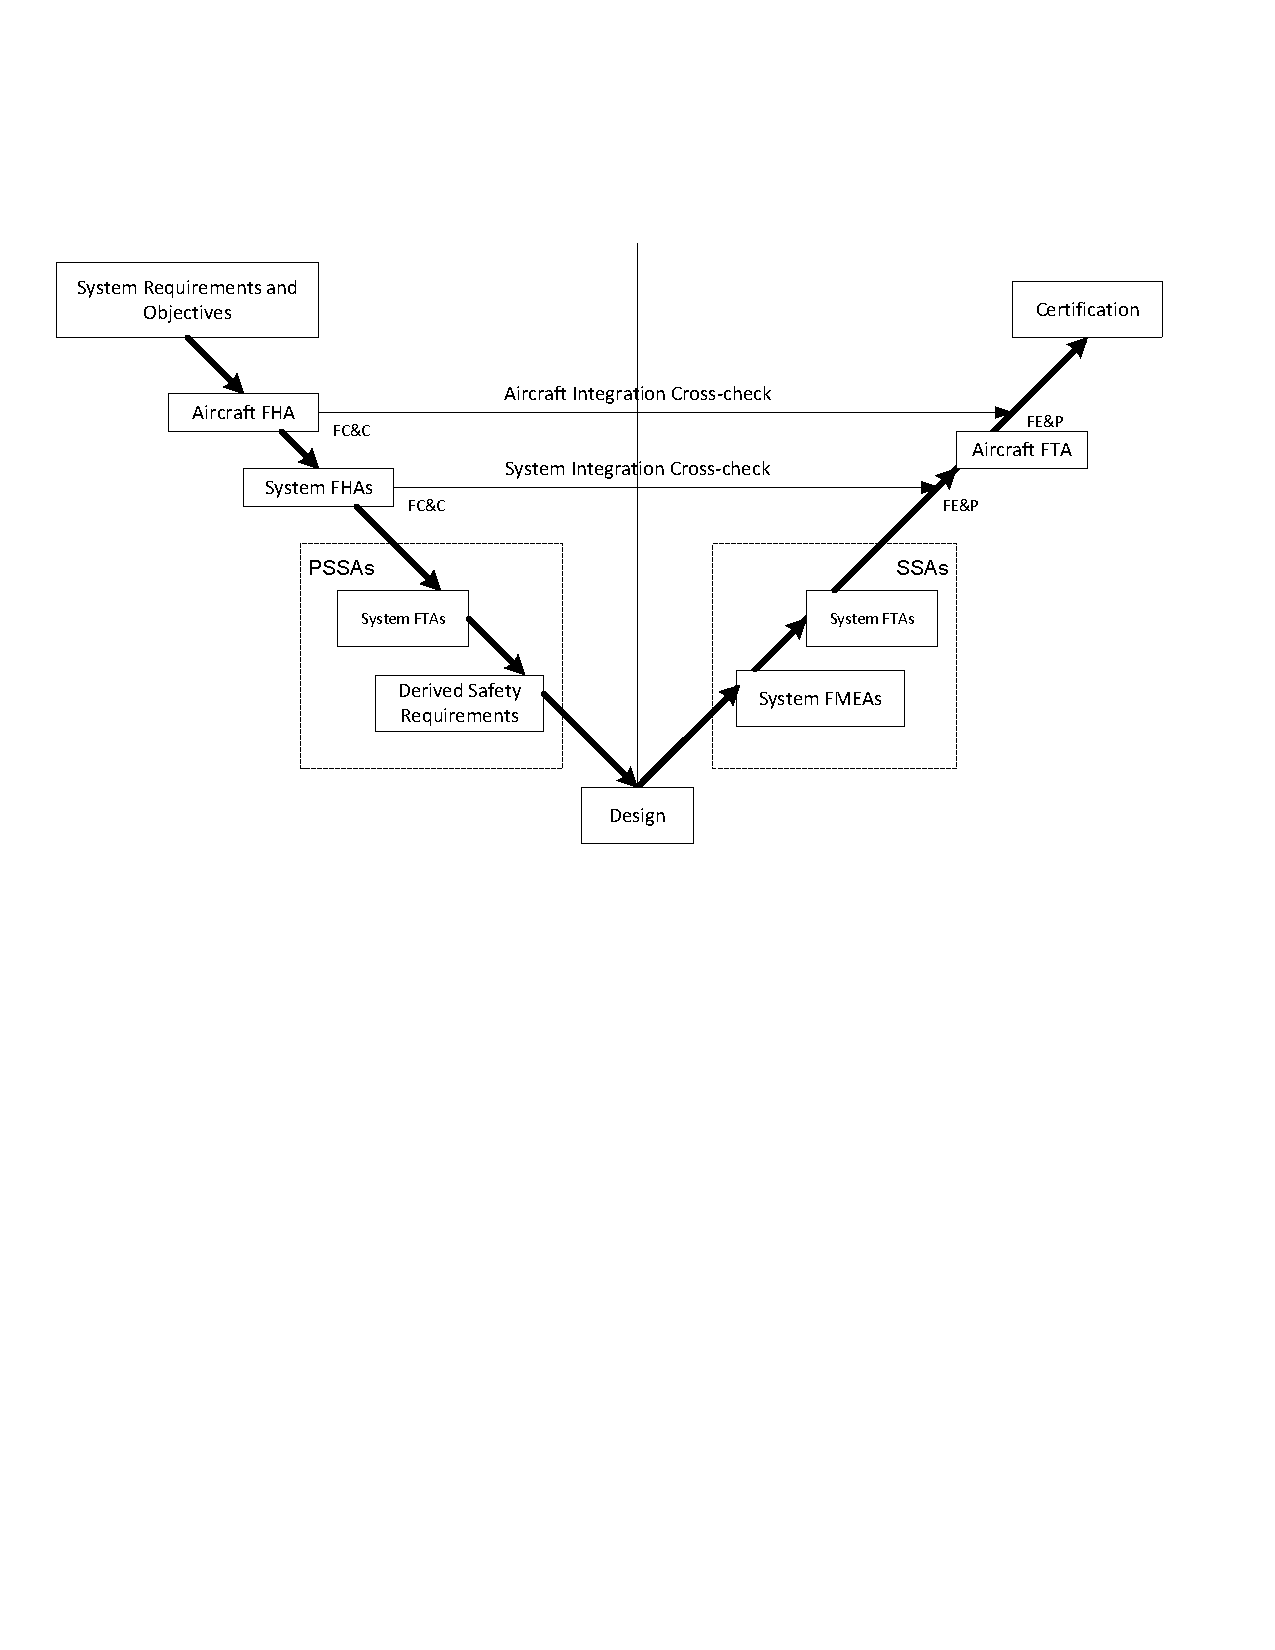
\includegraphics[trim=25 375 0 125, clip, scale=.60]{V}
\caption{Traditional ``V'' Safety Assessment Process} \label{fig:V}
\end{figure}

%The safety assessment process is an integral part of the development process.

Figure~\ref{fig:V} from \cite{Joshi05:SafeComp} shows an overview of the safety assessment
process as recommended in ARP 4761. The process includes safety
requirements identification (the left side of the ``V'' diagram)
and verification (the right side of the ``V'' diagram), that
support the aircraft development activities. An aircraft level
Functional Hazard Analysis (FHA) is conducted at the beginning of
the aircraft development cycle, which is then followed by system
level FHA for individual sub-systems. The FHA is followed by
Preliminary System Safety Assessment (PSSA), which derives safety
requirements for the subsystems, primarily using Fault Tree
Analysis (FTA). The PSSA process iterates with the design
evolution, with design changes necessitating changes to the
derived system requirements (and also to the fault trees) and
potential safety problems identified through the PSSA leading to
design changes. Once design and implementation are completed, the
System Safety Assessment (SSA) process verifies whether the safety
requirements are met in the implemented design. The system Failure
Modes and Effects Analysis (FMEA) is performed to compute the
actual failure probabilities on the items. The verification is
then completed through quantitative and qualitative analysis of
the fault trees created for the implemented design, first for the
subsystems and then for the integrated aircraft.

%\medskip

We propose to modify this traditional ``V'' process so that the
lower level PSSA and SSA activities are performed based on a
formal model of the system under consideration.
Figure~\ref{fig:Vmod} shows the modified ``V'' diagram for
model-based safety analysis. The shaded blocks are those
activities that will be modified or added.

\begin{figure}
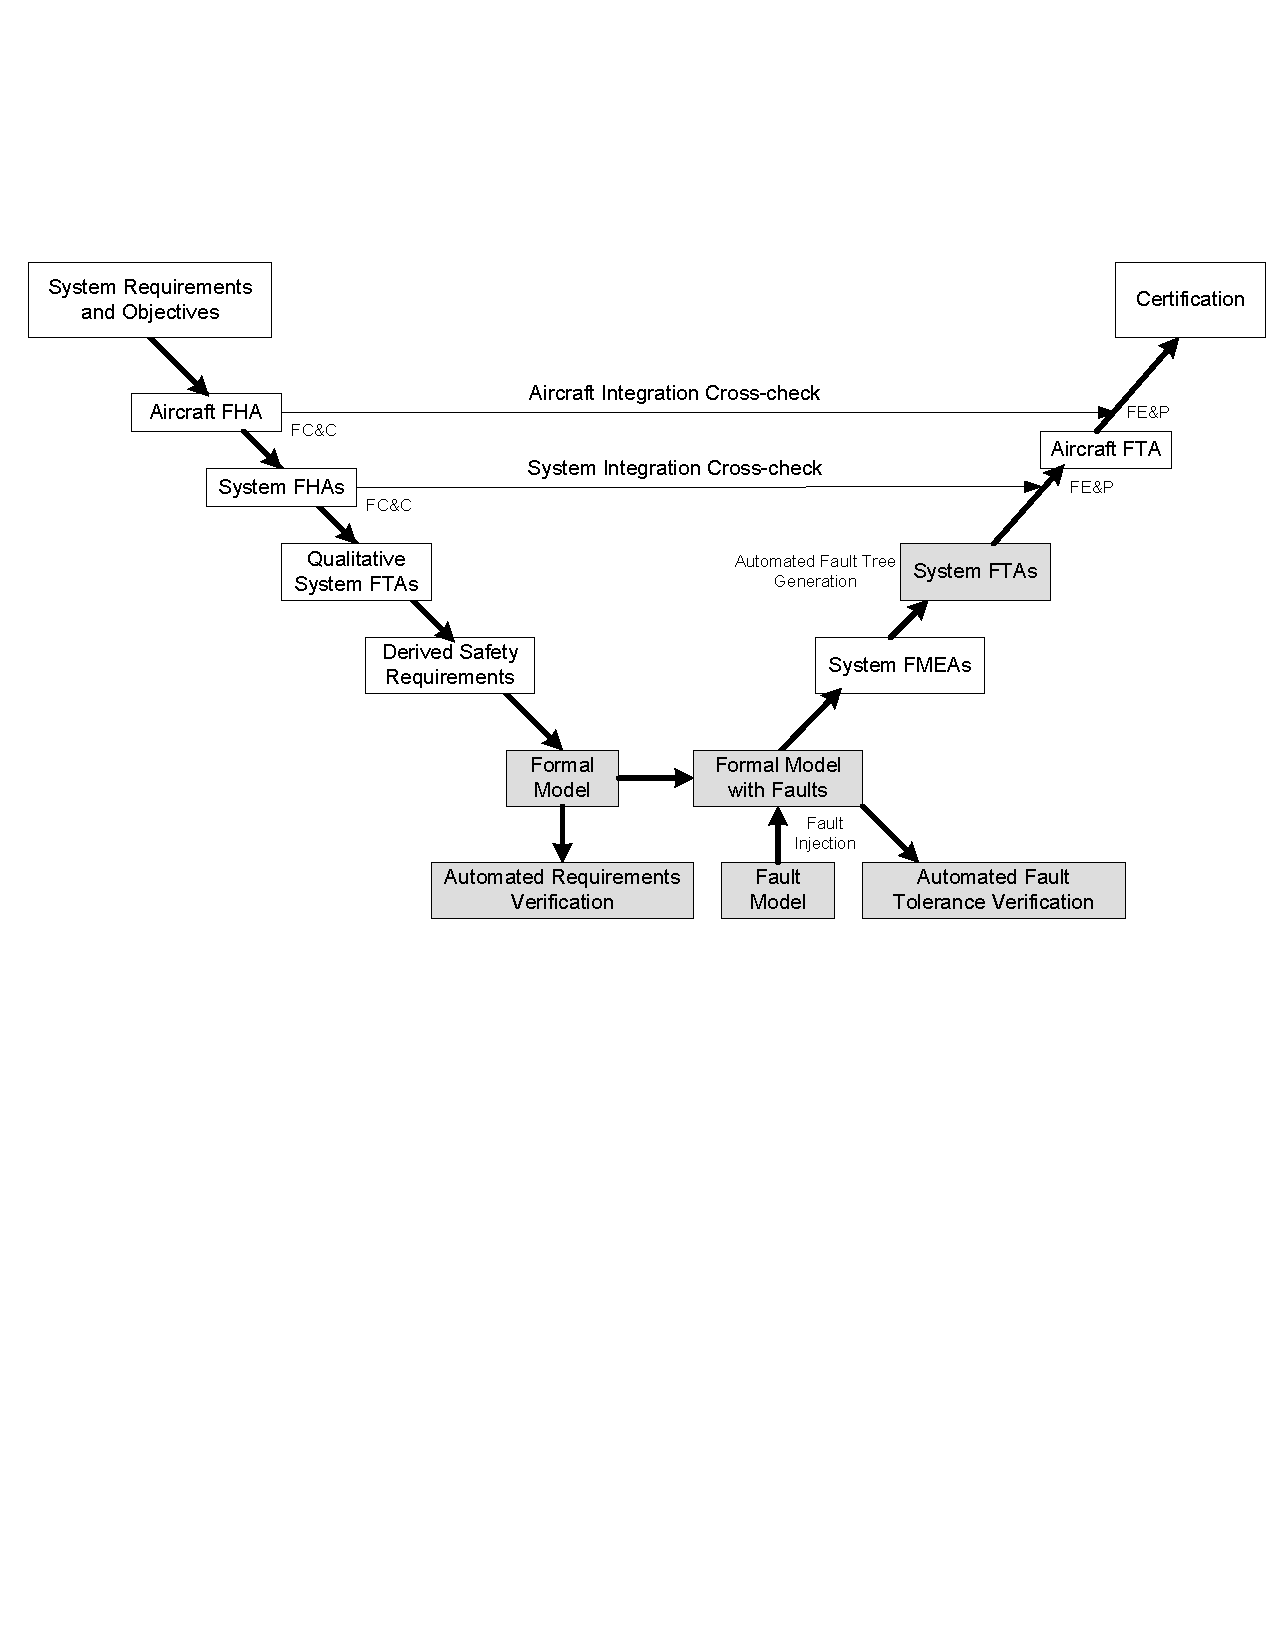
\includegraphics[trim=15 350 0 125, clip, scale=.60]{Mod_V_Process_FaultModel}
\caption{Modified ``V'' Safety Assessment Process} \label{fig:Vmod}
\end{figure}


As we can observe from Figure~\ref{fig:Vmod}, the parts of the analysis that are
primarily affected are at the bottom of the ``V''. The biggest difference is that
the safety analysis activities at this level are now focused around a formal
model of the system behavior, and that many of the artifacts of the safety
analysis can be derived from this model. The idea is to try to pose the right
verification questions to formal tools (such as model checkers and theorem
provers) so that it is possible to derive the necessary safety analysis
information. We then wish to turn the results of these analyses back into
artifacts that can be easily understood and used by safety engineers.


\section{Functionality}





\section{Architecture and Implementation}


The architecture of the safety annex plugin is shown in Figure~\ref{fig:plugin-arch}.  It is written in Java and is hosted in the OSATE AADL toolset, which is in turn built on Eclipse.  It is not designed as a stand-alone extension of the language, but to work with existing behavioral information in the {\em Assume-Guarantee Reasoning Environment} (AGREE) AADL annex and tools~\cite{NFM2012:CoGaMiWhLaLu}.  AGREE allows {\em assume-guarantee} behavioral contracts to be added to AADL components.  The language used for contract specification is based on the LUSTRE dataflow language~\cite{Halbwachs91:IEEE}. The tool allows scaling of formal verification to large systems by splitting the analysis of a complex system architecture into a collection of verification tasks that correspond to the structure of the architecture.

\begin{figure}
\begin{center}
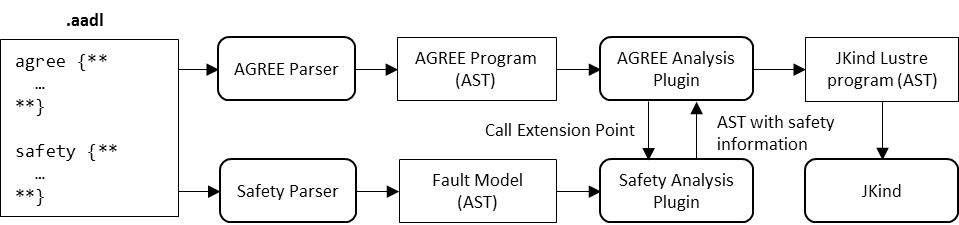
\includegraphics[trim=0 400 430 0,clip,width=0.85\textwidth]{images/arch.png}
\end{center}
\vspace{-0.2in}
\caption{Safety Annex Plug-in Architecture}
\label{fig:plugin-arch}
\end{figure}

AGREE contracts are normally used to define the nominal behaviors of system components as {\em guarantees} under {\em assumptions} about the values the component's environment will provide.  The safety annex extends these contracts to allow faults to modify the expected behavior of component inputs and outputs.  To allow for these kinds of extensions, AGREE implements an Eclipse extension point interface that allows other plug-ins to modify the generated AST prior to its submission to the solver.  If the safety annex is enabled, these faults are added to the AGREE contract and, when activated, override the normal guarantees provided by the component.  An example of a portion of an initial AGREE node and its extended contract is shown in Figure~\ref{fig:comp}.  The \texttt{\_\_fault} variables and declarations are added to allow the contract to override the nominal behavioral constraints (provided by guarantees) on outputs.  In the Lustre language, \texttt{assertion}s are constraints that are assumed to hold in the transition system.

\begin{figure}
\vspace{-0.1in}
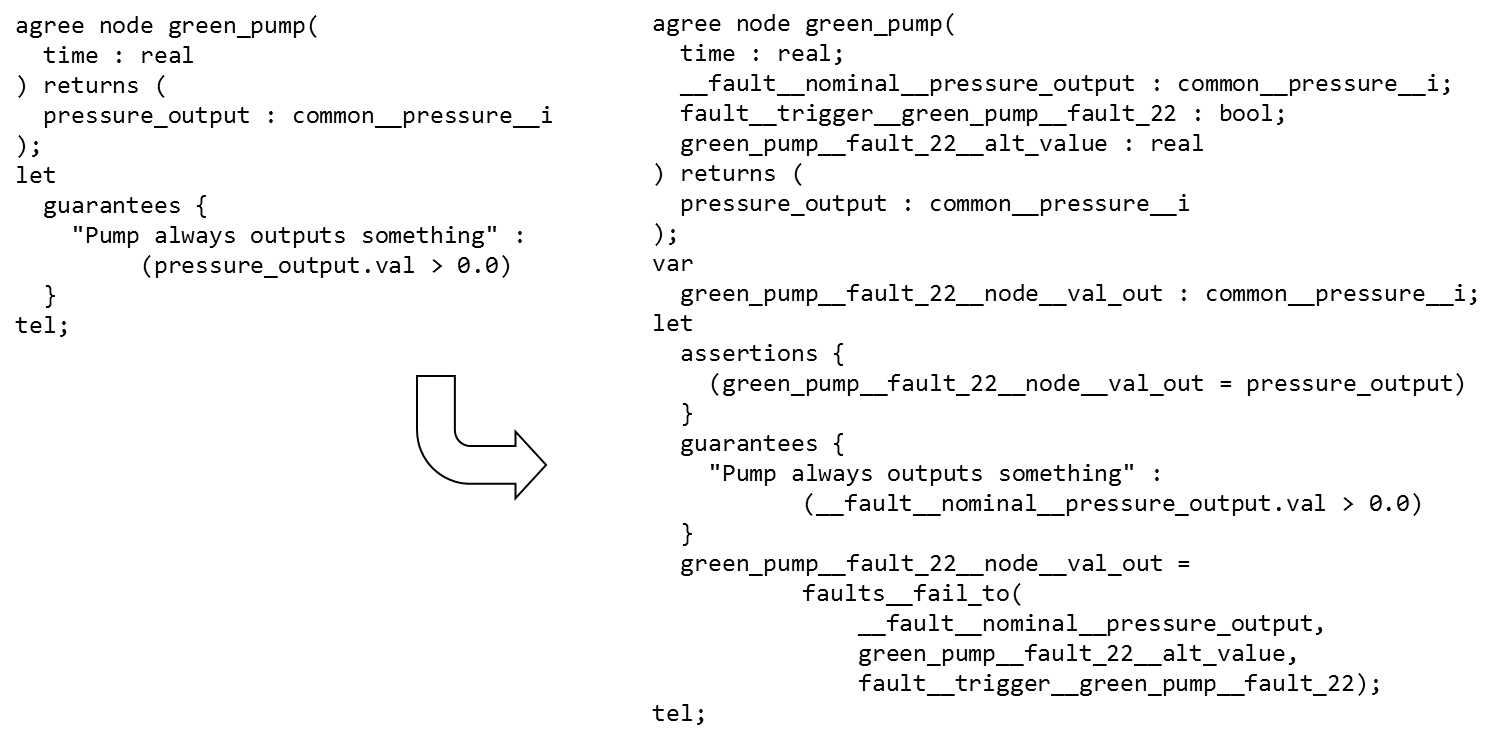
\includegraphics[trim=30 150 120 10,clip,width=\textwidth]{images/sample_code.png}
\vspace{-0.3in}
\caption{Nominal AGREE node and its extension with faults}
\label{fig:comp}
\end{figure}

An annotation in the AADL model determines the fault hypothesis: either that a maximal number of faults can be active at any point in execution (often one or two), or that only faults whose probability of simultaneous occurrence is above some probability threshold.  In the former case, we assert that the sum of the 'true' {\em fault\_\_trigger} variables is under some integer threshold.  In the latter, we determine all fault combinations of faults whose probabilities are above the specified probability threshold, and describe this as a proposition over {\em fault\_\_trigger} variables.

Once augmented with safety information, the AGREE model follows the standard AGREE translation path to the model checker JKind~\cite{2017arXiv171201222G}, an infinite-state model checker for safety properties.  The augmentation includes traceability information so that when counterexamples are displayed to users, the active faults for each component are visualized.





\section{Applications}

To evaluate the effectiveness of the Safety Annex, we updated the WBS model~\cite{Stewart17:IMBSA} to specify faulty component behaviors. The components' nominal  and faulty behaviors are modeled separately. At the top-level AADL component, the fault hypothesis was specified as the maximum number of faults that can be active at any time. The AGREE contracts at the top-level component were verified using AGREE, with the ``Perform Safety Analysis'' option selected. The tool automatically weaves the nominal and faulty behaviors before feeding the result to the model checker.

In this example, the top level contract ``Pedal pressed and no skid implies brake pressure applied'' was verified in the presence of at most one fault active during execution.  However, it was shown to be invalid when more than one fault was allowed. The counterexample indicated that both Selector's outputs failed to non-deterministic values due to the faults introduced.

We also applied the Safety Annex to the Quad-Redundant Flight Control System (QFCS) model~\cite{QFCS15:backes}.  We introduced faulty behaviors to see the response of the system to several faults, and to evaluate fault mitigation logic in the model.  The QFCS system-level properties failed when unhandled faulty behaviors were introduced.

We also used the Safety Annex to explore more complicated faults at the system level on a simplified QFCS model with cross-channel communication between its Flight Control Computers.

\begin{itemize} 
	\item Byzantine faults~\cite{Driscoll-Byzantine-Fault} were simulated by creating one-to-one connections from the source to multiple observers so that disagreements could be introduced by injecting faults on individual outputs. A system-level property failed due to the fault on the baseline model, but did not fail on the model with Byzantine fault handling protocol added. Using the Safety Annex like this can test a system's vulnerability to Byzantine faults and verify mitigation mechanisms.
	
	\item Dependent faults in hardware were simulated by injecting faults to hardware components (physical layer) to affect their data outputs (logical layer), and consequently failing the software components bound to the hardware components. The relationship between the hardware components' outputs and the software components' inputs were specified in AGREE as part of the system's nominal behavior.	
\end{itemize}




















\section{Conclusion}

We have developed an extension to the AADL language with tool support for formal analysis of system safety properties in the presence of faults. Faulty behavior is specified as an extension of the nominal model, allowing safety analysis and system implementation to be driven from a single common model. This new Safety Annex leverages the AADL structural model and nominal behavioral specification (using the AGREE annex) to propagate faulty component behaviors without the need to add separate propagation specifications to the model.   Next steps will include extensions to automate injection of Byzantine faults as well as automatic generation of fault trees.  For more details on the tool, models, and approach, see the technical report~\cite{SATechReport}.

\vspace{2 mm}
\noindent {\bf Acknowledgments.} This research was funded by NASA contract NNL16AB07T and the University of Minnesota College of Science and Engineering Graduate Fellowship.



%ACKNOWLEDGMENTS are optional
%TODO: Fill in for final version
\vspace{0.08in}


%\textbf{Acknowledgments:}
%This work was supported by

%We thank XXXX

\bibliographystyle{abbrv}
\bibliography{biblio}

% This ~ seems to fix an odd bibliography alignment issue
~

%\ifdefined\TECHREPORT
%\appendix
%
%\section{Appendix: Proof of Equivalence}
%\input{appendix}
%\fi

%\section{Appendix: GPCA CENTA Model}
%\label{appendix:gpcacenta}
%\begin{figure}[!ht]
%\begin{center}
%\includegraphics[scale=0.6]{images/sampled_pca.PNG} %[trim = 0 2 0 0, clip=true]{Comp}
%\caption{GPCA AGREE Properties modeled as a Timed Automata} \label{fig:samplepca}
%\end{center}
%\end{figure}

%\balancecolumns

\end{document}
